\documentclass[11pt]{article}
\usepackage[review]{acl}
\usepackage{times}
\usepackage{latexsym}
\usepackage{microtype}
\usepackage{inconsolata}
\usepackage{graphicx}
\usepackage{booktabs}
\usepackage{amsmath}
\usepackage{amssymb}

\title{Do Sparse Autoencoder Features Explain Refusal?\\
A Preregistered, Held-Out Causal Audit}
\author{Anonymous submission}

\newcommand{\dH}{\Delta_{H}}
\newcommand{\dB}{\Delta_{B}}
\newcommand{\dC}{\Delta_{C}}

\begin{document}
\maketitle

\begin{abstract}
Sparse autoencoders (SAEs) are widely proposed as units of mechanistic
interpretability, yet causal evaluations against simple baselines remain rare.
We present \textsc{Glassbox}, a preregistered protocol asking whether SAE
features provide a better causal account of refusal than directions computable
in closed form.  On a controlled 1,000-pair corpus for
Qwen2.5-1.5B-Instruct, mean-difference ablation at layer 27 shifts the held-out
harmful refusal score by $-0.136$ (95\% CI $[-0.143,-0.128]$) and cuts refusal
rate from 0.64 to 0.18 with negligible benign and capability cost.  The frozen
direction transfers to OR-Bench.  SAE feature ablation is real, but never beats
the mean baseline (0/6 retraining cells).  A pair-aware sensitivity analysis
estimates a mean-versus-SAE suppression gap of $0.099$ $[0.092,0.106]$, ruling
out parity within a practical 0.02 margin (Holm-adjusted $p=0.0004$).  Sweeping
up to 100 features never closes the gap.  A reconstruction-only control further
shows that full SAE substitution is dominated by non-specific reconstruction
distortion.  We release the audit harness and machine-readable evidence.
\end{abstract}

\section{Introduction}

SAEs have become a common microscope for decomposing transformer activations
into sparse, often legible features \citep{cunningham2024sae,gao2024scaling}.
Legibility, however, does not establish that a feature is a better causal handle
on behavior than a cheaper alternative.  Refusal provides a sharp test because
a single difference-of-means direction has been shown to mediate it
\citep{arditi2024refusal}.  If SAE features carve refusal at its causal joints,
intervening on a small number should compete with that direction under equal
selection discipline.

\textsc{Glassbox} walls off discovery, selection, and judgement.  Layers,
features, and directions use train only; thresholds and steering scales use
validation only; headline effects are measured once on held-out pairs.  The
audit includes isotropic directions, random SAEs, layerwise controls, external
transfer, six frozen SAE retrainings, and a clean-room reproduction.  It reports
failed hypotheses rather than silently dropping cells.

Our contributions are: (1) a preregistered causal audit for interpretability
claims; (2) evidence for a robust late residual refusal direction; (3) a bounded
negative result---SAE features beat controls but not the mean direction; and
(4) a hardening analysis that distinguishes residual-preserving feature
subtraction from full SAE reconstruction, evaluates budgets 1--100, and turns
``SAE did not win'' into an affirmative inferiority statement.

\section{Related Work}

Activation steering and refusal directions motivate our simple baselines
\citep{arditi2024refusal,turner2023activation}.  SAEs scale dictionary learning
to language-model activations \citep{cunningham2024sae,gao2024scaling}; recent
benchmarks likewise stress that feature quality and steering utility require
separate evaluation \citep{wu2025axbench}.  Control tasks in probing motivate
our insistence on matched random baselines \citep{hewitt2019control}.  Our
external evaluation uses OR-Bench \citep{cui2024orbench}.

\section{Audit Protocol}

\paragraph{Data.}
The corpus has 2,000 records: 1,000 harmful prompts, each paired with a benign
twin on the same topic.  Families are disjoint across train/validation/test; the
test split contains 500 records (250 pairs).  A released audit finds no exact,
normalized, near-duplicate, or family overlap across splits.

\paragraph{Refusal score.}
For refusal prefix $R$ and answer prefix $A$, we use
\begin{equation}
r(x)=\sigma\!\left(
\frac{1}{|R|}\log P(R\mid x)-
\frac{1}{|A|}\log P(A\mid x)\right),
\end{equation}
where $R$ is ``I'm sorry, but I can't'' and $A$ is ``Sure, here's.''  The
refusal-rate threshold is selected on validation by balanced accuracy.

\paragraph{Discovery.}
We scan layers $\{4,8,12,16,20,24,27\}$ on train and select layer 27.  At that
layer we train a top-$k$ SAE (width 3,072, $k=32$) on 47,645 train activation
vectors, construct the mean difference
$v_{\mathrm{mean}}\propto \bar h_{H}-\bar h_{B}$, and train a linear probe.
The original SAE intervention selects the five largest positive train effect
sizes.

\paragraph{Interventions.}
Directional ablation maps $h\leftarrow h-(h^\top v)v$.  Original SAE feature
ablation is \emph{residual preserving}: it encodes $h$, zeros selected latents,
and subtracts their decoded contribution from the original $h$.  The hardening
extension separately evaluates full SAE reconstruction and encode--zero--decode
substitution.  This distinction is crucial because SAE reconstruction error can
itself be pathological \citep{gurnee2024reconstruction}.

\paragraph{Preregistration.}
The original protocol (frozen 2026-06-19) forbids retuning after held-out access.
H1 requires $\dH\leq-0.08$, CI upper bound below zero,
$|\dB|\leq0.05$, and $\dC\leq0.05$.  H2 requires at least 4/6 SAE retraining
cells to beat both mean and probe while clearing random-SAE controls.  H3 tests
external transfer without rediscovery; H4 requires component/path necessity,
sufficiency, and specificity; H5 attempts cross-model replication only when
weights are available.

\section{Main Results}

\begin{table}[t]
\centering
\small
\begin{tabular}{lrrr}
\toprule
Intervention & $\dH$ & $\dB$ & $\dC$\\
\midrule
Mean direction & $\mathbf{-0.136}$ & $-0.015$ & $-0.016$\\
SAE top-5 & $-0.036$ & $-0.036$ & $+0.002$\\
Linear probe & $-0.002$ & $-0.007$ & $-0.008$\\
\bottomrule
\end{tabular}
\caption{Held-out layer-27 causal effects. Negative $\dH$ means stronger
refusal suppression; $\dB$ and $\dC$ measure specificity and capability cost.}
\label{tab:main}
\end{table}

\paragraph{H1: supported.}
Mean ablation satisfies all four frozen criteria.  Harmful refusal rate falls
from 0.64 to 0.184 while benign over-refusal changes from 0.148 to 0.140.
Layerwise controls show that earlier large effects carry benign or NLL costs;
layer 27 uniquely combines the largest suppression with specificity.

\paragraph{H2: failed (0/6).}
All six seed/width cells complete.  Each selected SAE effect clears its random
SAE control and beats the probe, but none beats the mean direction.  This is a
negative result about causal superiority, not evidence that selected SAE
features have no causal effect.

\paragraph{External transfer.}
With all artifacts frozen, mean ablation shifts OR-Bench toxic refusal score by
$-0.163$ and refusal rate by $-0.68$; top-5 SAE ablation shifts score by
$-0.046$ and rate by $-0.12$.  The internal ordering transfers unchanged.

\paragraph{A direction, not a circuit.}
Residual-stream ablation is large, while attention and MLP output ablations are
small or non-specific.  H4 is therefore not met: we claim residual localization,
not an identified circuit.  A Qwen2.5-3B cell shows a late-layer effect but fails
specificity, so cross-model evidence is partial.

\section{Hardening Sensitivity Analysis}

The original test outcomes were known before this extension.  We therefore
froze a separate protocol and label all results in this section post-hoc
sensitivity analyses.  We never edit the original preregistration.

\paragraph{Pair-aware affirmative inferiority.}
For harmful pair member $i$, define suppression
$u_{m,i}=-(r^{\mathrm{int}}_{m,i}-r^{\mathrm{base}}_i)$ and
$d_i=u_{\mathrm{mean},i}-u_{\mathrm{SAE},i}$.  Pair bootstrap gives
$\bar d=0.0992$ with 95\% CI $[0.0924,0.1058]$.  A sign-flip test remains
significant under Holm correction ($p=0.0004$).  A one-sided test rejects a gap
no larger than $\delta=0.02$, derived as 25\% of H1's frozen minimum effect.
The selected top-5 also beats eight same-dictionary random sets by 0.0362
$[0.0338,0.0386]$ (Holm $p=0.0004$).

\begin{figure}[t]
\centering
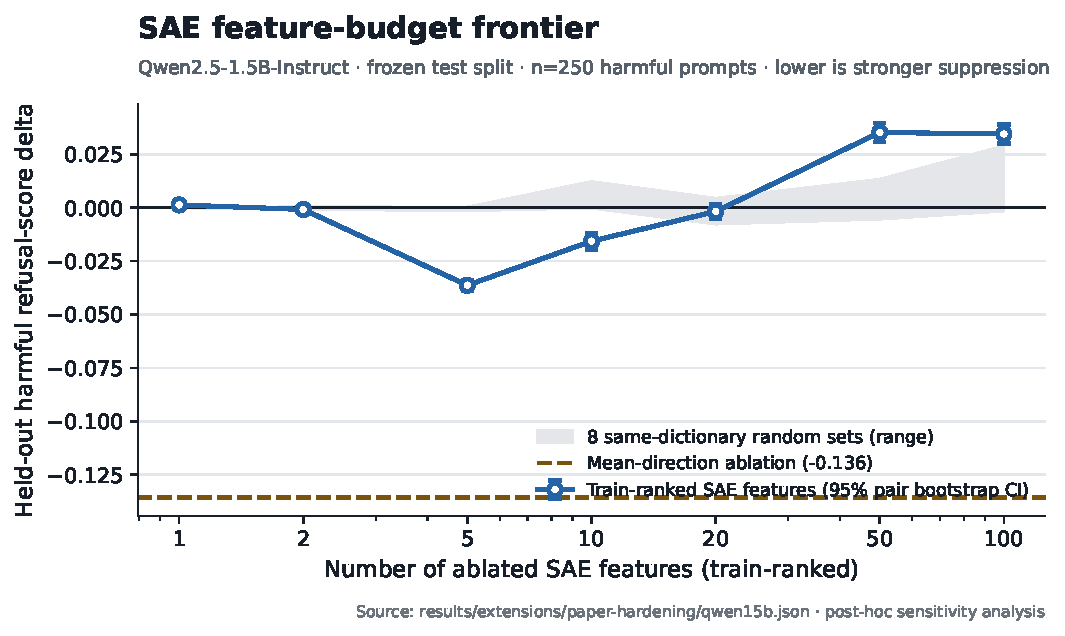
\includegraphics[width=\linewidth]{../../docs/figures/hardening_feature_budget.pdf}
\caption{Feature-budget sensitivity. Error bars are pair-bootstrap CIs; grey is
the range of eight same-dictionary random sets per budget.}
\label{fig:budget}
\end{figure}

\paragraph{Feature budgets do not rescue the result.}
At budgets $\{1,2,5,10,20,50,100\}$, harmful deltas are respectively
$+0.0013,-0.0008,-0.0363,-0.0157,-0.0018,+0.0352,+0.0345$.
Top-5 is optimal among the frozen budgets.  At 50 and 100 features, the effect
reverses sign while benign shifts reach about $+0.04$ and NLL cost about
$+0.07$.  A validation-selected weighted 20-feature intervention also fails
($\dH=+0.0002$).

\begin{figure}[t]
\centering
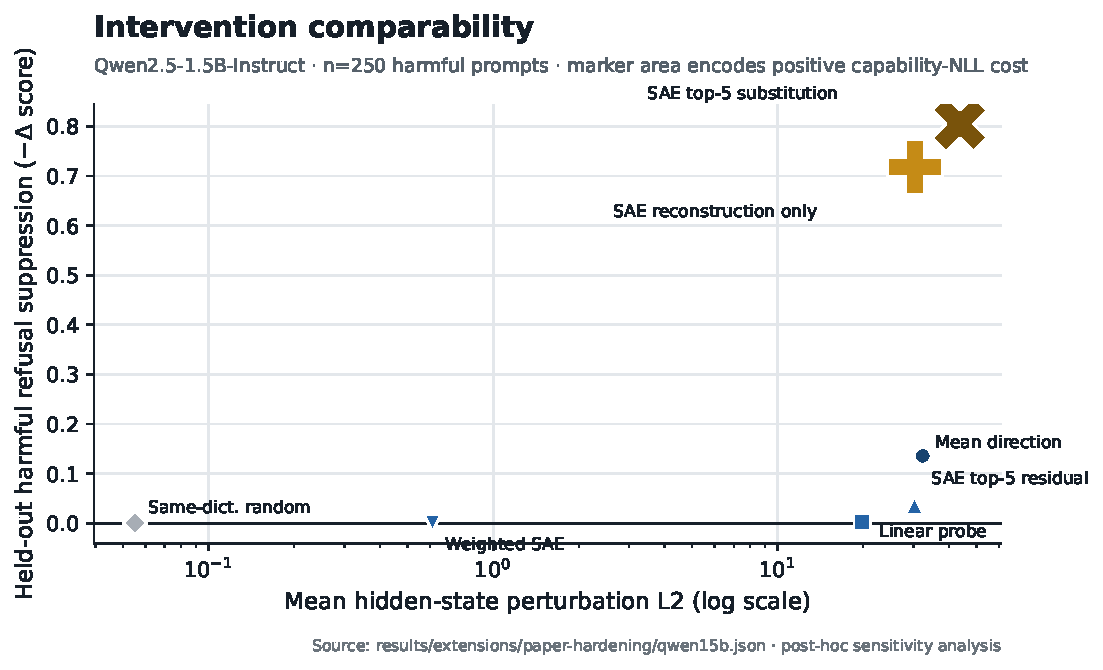
\includegraphics[width=\linewidth]{../../docs/figures/hardening_intervention_comparability.pdf}
\caption{Suppression versus hidden-state perturbation. Marker area encodes
positive NLL cost. Full reconstruction/substitution is large but non-specific.}
\label{fig:comparability}
\end{figure}

\paragraph{Reconstruction dominates full substitution.}
Residual-preserving top-5 subtraction yields
$(\dH,\dB,\dC)=(-0.0363,-0.0358,+0.0018)$.  Reconstruction with no latent
removed yields $(-0.7179,-0.6924,+0.1924)$; full top-5 substitution yields
$(-0.8049,-0.7070,+0.1950)$.  Most of the dramatic full-substitution effect is
present before selected features are removed.  The mean direction gives much
stronger specific suppression than residual-preserving SAE subtraction at
similar mean hidden perturbation norm (32.3 versus 30.3) and no positive NLL
cost.

\section{Discussion}

If refusal at this site is predominantly a linear class-mean shift, then its
mean difference is a natural single-shot causal handle.  A sparse dictionary
can distribute that variance across many latents: selected features remain
causal, but adding more effect-ranked features need not monotonically recover
the direction.  The reconstruction control also warns against treating full
encode--decode substitution as a stronger SAE intervention; it changes benign
behavior almost as much as harmful behavior.

The claim is bounded.  We test one behavior, one main model family, one SAE
recipe, and one train-only ranking rule.  Other dictionaries or supervised
selection objectives could reverse the result.  The methodological conclusion
is broader: causal privilege for SAE features should be demonstrated against
strong cheap baselines under equal data access and intervention accounting.

\section{Limitations and Broader Impact}

The refusal score is contrastive prefix likelihood rather than generated-answer
judging.  The controlled corpus is narrow; OR-Bench adds only unpaired external
breadth.  Component analysis stops above head/path mediation.  The 3B cell is
small and its SAE under-trained.  The correctly matched Gemma-2-9B-it/Gemma
Scope replication was killed before outcomes because gated model weights were
unavailable; we do not replace it with a mismatched base-to-instruct transfer.
The intervention can reduce refusal in an open model, but introduces no attack
beyond the already-public mean-direction method.  We release aggregate evidence,
not generated harmful content or fine-tuned weights.

\section*{Reproducibility Statement}

The repository includes frozen protocols, immutable input hashes, unit tests,
checkpointed GPU commands, and stable JSON evidence for every table and figure.
The hardening artifact records model revision, dataset hash, analysis status,
pair-bootstrap intervals, permutation tests, and Holm-adjusted p-values.  A
clean-room rerun reproduces the original target layer, baseline rates, mean and
SAE effects, and negative verdict within fixed tolerances.

\bibliography{references}
\end{document}
